\section{Getting back on track}
% 13 pages
We will now describe how we plan to get the project back on its tracks.

Doing this is going to take a lot of planning. However, while planning can help structure the collaboration, it can also add quite a bit of overhead. Therefore, we must carefully select the extent of our planning, and the methods we want to use. And if we spend too much time planning, we might not meet the deadline because of it, and if we use to little time planning, everything might derail again.

In the following sections we will describe the methods used to get the project back on track. Where possible, we will reflect upon the results of using that particular method as well.

\subsection{Planning second half}
% 1 page
The best way to get the project back on track is through careful planning. First of all we needed to get an overview of the remaining parts of the project, and then we wanted to carefully structure and plan: What needs to be done?, In what order? and How much time do we have?

We have divided the planning up into four parts.

We start out by looking at the development methods that we want to use. We give a brief introduction to the method, and explain how we applied it, helping the project back on track

After this we describe the estimation methods we use. The estimation methods should help us make accurate estimations. This, in turn, helps us to meet deadline, as most of our estimations should be correct or close to.

Now that we have found out how much time we need, we need to find out how much time we have available. For this we use a couple of methods for planning the time. Those methods are explained, and our usage is analyzed.

As the last, but most important part, we look into how our save of the product has affected the quality. Less time to do roughly the same work must have some effect on quality. This is analyzed.
% !TeX spellcheck = en_US
\subsection{Method of development}
% 3 pages
In the first part of the project, we entirely decided against using SCRUM because the project and its environment did not allow us to perform all practices dictated by SCRUM. The result was an unstructured development process leading to all kinds of problems.
We do like the SCRUM development method, however, and in this part of the project we will attempt to take a more gradual approach to SCRUM. The project and its environment is still not ideal for full SCRUM, but instead of rejecting SCRUM entirely, we will only reject those parts that are not well suited for the project.

A SCRUM activity we have chosen to exclude among others is the Daily SCRUM meeting.
At the Daily SCRUM meeting the development team and the SCRUM-master is updated with progress and set-backs.
We are a small group of only 5 people, however, and we do not have people to fill out all roles used in proper SCRUM, such as product owner and stake holders - we are only able to represent the development team.
As development will be done with the group assembled, we see no need for spending 15 minutes every meeting updating each other, as we already do this ad hoc when we are working.
The API we have defined and the SCRUM backlog should be enough to make the progress visible to all team members. Any problem which may arise during development may be discussed in plenum immediately.

\begin{figure}[t]
  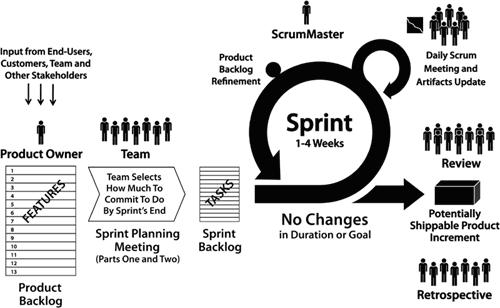
\includegraphics[width=\textwidth]{illustrations/scrum.jpg}
  \caption{An overview of SCRUM and its many activities. Of the displayed practices we have decided to use only the product backlog. Source: [\textit{http://softlinksolutions.com/development\_methodology.aspx}]}
  \label{scrum_picture}
\end{figure}

As just mentioned, we have decided to use a backlog, which is another SCRUM artifact.
The backlog is a prioritized list of items, where each item describes a program feature, often called a `story', possibly with sub-tasks that needs to be completed. Traditionally the product owner defines the order of the items, putting the features he wants implemented first at the top of the list \cite[p. 12]{scrum-org-guide}.
We have chosen to use a backlog as it ensures that the most vital functionality is implemented before less important, nice-to-have features. We will also benefit from producing the backlog itself, as we will be forced into enumerating all features to implement, giving us an overview of the work and ensuring that no big task suddenly pops up later.
Our complete backlog can be viewed in \atref{backlog}.

We have chosen not to divide our project into sprints, even though they are a core foundation of SCRUM.
Sprints are great for projects with longer time spans than ours, as it divides the project into smaller iterations, each producing valuable functionality able to function on its own, making it easier to keep focus.
After every sprint, the SCRUM team do a review, a retrospective, and plan which backlog items to implement during for the next sprint \cite[p. 8]{scrum-org-guide}.
Were we to divide our project into sprints, it would be very short ones, and it would not be worth the overhead from managing sprint backlogs and do reviews and retrospectives.

During a sprint, a SCRUM Task Board artifact is used to maintain overview of the sprint progress. The board is divided into four parts (`not started',`in progress', `to test' and `complete') with each task of the sprint listed under the appropriate section.
When a task is started it is moved from `not started' to `in progress', when a task is finished it is moved to `to test', and when it has passed its tests it is moved to `complete'.
Often a physical board is used so everyone, all the time, is able to keep track of the progress. This however, is only possible if all team members are at the same location, and it may be difficult to do, if the team cannot persist the board between sessions, for instance if the work location changes for each meeting.
For our project we have found a way to deploy a task board with minimum overhead by using a software version, always allowing every team member to keep track of the project wherever they are. Since we do not use sprints, the task board will give an overview of the progress of the whole project and of the individual tasks.\\
Our task board can be viewed in \acref{taskboard}. \textbf{[ TODO: Insert in appendix ]}

The burndown chart in SCRUM (as well as in other measurable environments) is used to monitor the progress of remaining tasks - in SCRUM this is the sprint backlog.
The burndown chart is a basic diagram where the y-axis symbolizes the remaining work and the x-axis symbolizes the remaining time to complete the work.
When the sprint is started a diagonal line is drawn from $(0, y)$ to $(x, 0)$, where $y$ is the amount of work and $x$ is the amount of time.
Each day the progress is plotted in with a line, which shows the current status, and thereby maybe even the effectiveness of the team. If the latest progress line ends below or at the diagonal line, the project is progressing well; if not, the project is progressing too slowly, and the sprint will not be completed in time with all planned features.
Since our project effectively is a "one sprint"-project, we will use the burndown chart to measure whether we are on track or are falling behind schedule.\\
Our burndown chart can be viewed in \acref{burndown}. \textbf{[ TODO: Insert in appendix ]}

To perform and maintain the various artifacts described above, we have chosen to use scrumwise.com for all SCRUM related work. Our overhead from using SCRUM will be reduced, since the artifacts automatically will be updated whenever progress or changes are made to the backlog tasks.
Because the artifacts automatically are updated and always will be up to date, the site will easily allow us to monitor our progress and maintain our overview. Should our work not progress as estimated and planned, we will be able to spot it immediately, and may then pause our work to re-evaluate our plans, possible doing re-estimation of some or all of the tasks.

\subsection{Estimation methods}
% 3 pages
In the following we will present the methods we have used to estimate our tasks for the project. We will argue for not using certain other methods, and our thoughts on how we experienced the use of these methods.
\subsubsection{Planning Poker}
There exist multiple estimation methods, but for this (part of the) project, we have chosen to use Planning Poker, also know as Scrum Poker, to estimate the remaining tasks. Planning Poker is a good practice when using Scrum, and in a sense to use the WBS/PBS paradigm (in Scrum the backlog).

Planning Poker seemed like a good choice since we all have worked with Scrum before, but not used Planning Poker, so this was a great opportunity to practice it. Also the fact that the players don't influence each other when estimating, but the game still facilitates shorts discussion is a great advantage. The fact that the `game' facilitates discussions is the reason for why we chose Planning Poker instead of the Delphi estimation method, which does not. The discussion might not always be an advantage, though. It can easily become very time consuming. We chose a non-voting, but overruling, moderator to address this potential problem, and it worked perfectly and it was an advantage multiple times.\\
We could quite quickly ignore the Analogy method since it uses comparison of similar project, which we have not done before, hence it was not an option.

We made playing cards with the numbers 1/2, 1, 2, 3, 5, 8, 13, 21, 34, 55, 89, "?" and "break". The numbers represented man hours and the question-mark represented that the "player" was unsure about the amount of work in the task, and the "break" card represented that the player needed a short break from the game.\\
We found that using Planning poker was a great advantages compared to what we previously have done. Beside the work-related advantages we also found it way more motivating than other methods, and all members of the group was included in the process. Yet, the high numbers (34, 55 and 89) was never used, as well as the "break" card. The "?" was only rarely used, and almost not considered a valid card by the team, due to the fact when playing the card the player did not participate in the discussion. Also there where the risk of only one person having a real estimation vote for the task.

\textbf{Vi skal komme ind på CoCoMo og PERT-estimering}
\subsection{Methods for planning the time}
% 3 pages
Planning time on a project that has derailed can be considered the most important thing, although it depends on the other activities in order to be applied with success.

In the following we will describe the methods we have applied to the project, along with a single method which was considered, but was not deemed beneficial and hence not applied.

\subsubsection{Time schedule}
To be able to plan our time efficiently, we had to find out how much time we had at our disposal. Our way of doing this was to create a custom spreadsheet, containing all the dates until deadline. For each date a field for each person was present. In this field the hours available should be entered. This way it was easy for us to get an overview of when we all were available. This helped us a lot in planning our meetings.

Generally, we have decided, that if three or more group-members are available, a meeting should be planned. We would rather be done with everything before time, than only plan the hours that we needed to complete the backlog items

-- Insert diagram here --

Figure x shows our custom spreadsheet using this custom method. We have really had great benefit from doing it this way, as planning group meetings just was instant, without too much communication back and forth.

Whenever three or more group members had placed available hours in the same timespan on a specific date, we would plan a group meeting at that specific time. This meant that we had more group meetings than needed, but this also helped us meet our deadline on time.
\subsubsection{Dependency network with activity durations}
After planning all our group meetings we decided that a dependency network with activity durations. We have several reasons for doing this
\begin{itemize}
	\item We wanted to make sure that everyone always knew what to do. A dependency network is great for this purpose, as everyone can easily see which elements must precede others.
	\item We wanted to be able to quickly identify the critical path. We want this to make sure that minimum slack is applied to this path. To keep project on deadline.
	\item To be able to quickly see possible slack to backlog items. This helped us very much in determining which items to complete first.
\end{itemize}

-- Insert diagram here --

The above network shows our dependency network.
Some important parts to point out that we learned from this network:
\begin{itemize}
	\item It shows that testing WCF controller can be pushed all the way to the 73rd hour. We suspected that this part was not that important, but the network really confirmed us in this suspicion.
	\item It shows that we have to begin programming the controllers/models before views. But it does also show that not all controllers/models need to be finished before all of the views can be implemented. It should exactly which controllers/models that needs to be finished.
\end{itemize}

The network has helped us a lot in our work, and we have returned to it many times throughout the project.
\subsubsection{GANTT diagram}
A GANTT diagram can be an extremely efficient tool for planning in larger groups. Some overhead must be expected, but it gives an excellent overview of when activities should start, be finished, and how they should be carried out in relation to each other.

The overhead from using a GANTT diagram can be caused by the fact that you create an order in which the program should be created. We want it to be agile enough to be able to switch between items as we like.

We had spent a lot of time constructing a thorough dependency network, and we decided to use this alone, as the base of doing items. We agreed that the dependency network provided the right overview of our items.

Because we had a project that was derailed, we feared that the overhead applied by using a GANTT diagram would be too high, compared to the benefit gained from it. The benefit would also be minimal, because of our extensive dependency network.
\subsection{Quality assurance}
To be able to measure the quality of our client we use the requirements we set to the client along with a test strategy to ensure as little errors as possible and the methods descriped earlier in this chapter. We move from the initial level of Capability Maturity Model while developing the server to the managed level during the development of the client. We kept to the initial level during the development of the server, by developing as we went along.

The usage of a test strategy, increases the likelyhood of finding errors early and correcting them, thereby minimizing the amount of time on debugging. When we define the test criteria, combined with the product requirements, we get one way of measurering quality.

 If the product fulfills the requirements and pass the tests, depending on the tests, its reliability has been proved as well. Which is one of CISQ's 5 major desirable characteristics. The other 4 are; efficiency, security, maintainablility and size. The efficiency parameter comes partly from our planning and software design and partly from our implementation. Our software design encourages implementation of efficient code,

 
%\subsection{Summary}
%First step was to plan the rest of the project. We used the SCRUM artifact Backlog to get an overview. We estimated work hours for each item on the backlog, to further enhance our overview. This gave us an estimate of the number of remaining hours. We also planned our available hours. Comparing our available working hours with the hours remaining in the project, showed us that we had just enough time, assuming our estimates rang true. ``The project is not derailed then?'' you might ask, and it was: We planned a lot more available hours in order to meet the project's remaining hours.
\newpage